\documentclass[12pt]{article}

% Language setting
% Replace `english' with e.g. `pathspanish' to change the document language
\usepackage[english]{babel}

% Set page size and margins
% Replace `letterpaper' with`a4paper' for UK/EU standard size
\usepackage[a4paper,top=2cm,bottom=2cm,left=3cm,right=3cm,marginparwidth=1.75cm]{geometry}

% Useful packages
\usepackage{amsmath}
\usepackage{graphicx}
\usepackage{subfig}
\usepackage[colorlinks=true, allcolors=black]{hyperref}

\begin{document}

%title
\title{\underline{Project report - AutoPylot}}
\date{March 2022}


\author{%
    \\
    Alexandre Girold\\
    Mickael Bobovitch \\
    Maxime Ellerbach \\
    Maxime Gay \\ \\
    Group: Autonomobile 
    }

\maketitle

\centerline{
\includegraphics[height=7cm]{../../logos/logo-transparent-black.png}}
\newpage

\tableofcontents
\newpage

\section{Introduction}

\subsection{Project presentation}
Autonomous vehicles and more specifically self-driving cars have grasp the attention of many people for good or ill. In this spirit, we have decided with the Autonomobile team to create our first ever project, AutoPylot. The name of our team is of course full of meaning in that regard. Autonomobile is a two-word name, the first one a French word for autonomous : "Autonome", the second one a French word for car : "Automobile". These two-word combined literally mean Autonomous car.\\

What is AutoPylot's goal ? 
Drive itself on a track and win races. It may, at first glance seem very simple but not everything is at it seems. Yet we will try to make it as easy to understand as possible, without omitting crucial information. To achieve our goal, we need to solve many other problems. Those problems can be separate into two distinct groups. \\

The first one would be the software part. Indeed, in this project we will need to learn and acquire certain skills, from teamwork to coding in different languages. With those newly acquired skills we will be able to bring machine learning to our car to make it drive itself. This leads use directly to our second part, the more tangible one : hardware. Indeed, as we will progress in our work, we will need to see the results of our work in real life condition. This means implementing our code to a functioning car which will be able to race on a track. \\

This project will lead by a team of four young developers, Maxime Ellerbach, Mickael Bobovitch, Maxime Gay and Alexandre Girold. In this project work will be divided equally amongst all of us, sometimes we will have to work together to achieve our very tight time frame. 

\subsection{Team members}

% Write a small paragraph about yourself, what you like, what you did in the past. Everything is valuable !
\subsubsection{Maxime Ellerbach}
I am a curious and learning hungry person, always happy to learn and collaborate with new people ! Programming, robotics and tinkering has always attracted me. Writing code and then seeing the results in real life is something that I find amazing ! I had multiple projects in this field : Lego Mindstorms, a robotic arm, more recently an autonomous car and even a simulator in unity to train even without a circuit at home ! Even if I know quite well the domain of autonomous cars, there is always something new to learn. I look forward working with this team full of hard-working people on such a fun project !

\subsubsection{Mickael Bobovitch}
Roses are red. Violets are blue. Unexpected “Mickael BOBOVITCH“ on line 32. Hello I am a French Student with Russian parents. Lived half of my life in Moscow. Passionate in web dev, servers, and business. Started programming at 13 years old. Created many projects. I like to learn everything, from AI, to UI, from Hardware to Software. Actually I am like OCaml, you need to know me well to appreciate me.

\subsubsection{Maxime Gay}
I am 18 years old,  and I am crazy about investment, finance and especially cryptocurrencies and blockchain. I already worked with a team on different Investment projects and during summer Jobs, but this is the first time that I am working on such a  project. Furthermore, I am a beginner in computer Science and autonomous car. However, I am impatient to learn new skills with this incredible team. 

\subsubsection{Alexandre Girold}
I am already getting old. I am 19 years of age, yet I am full of resources. I am delighted to be able to learn something new. There are many things which I enjoy from programming to geopolitics. I know this project will push me toward a better me and make great friends along the way. 

\subsection{State of the art}
In this section, we will try to see what was previously made in this sector of industry.
It would not be realistic to compare our 1:10 project to real sized cars such as Tesla's, simply because in a racing environment,
we don't need to deal with such an amount of safety: pedestrian detection, emergency braking, speed limit detection and other.
So we will only see miniature autonomous racing framework that we would likely race against.\\

The most known is called "DonkeyCar", created by Will Roscoe and Adam Conway in early of 2017. Most of the models trained with DonkeyCar are behavior cloning models, meaning models that tries to replicate the behavior of a driver. This method uses a big amount of images (input) associated to steering angles and throttle (output), it requires the user to drive the car (collect data) prior to training the model: no examples means no training. The lack of training data often leads to the car leaving the track.\\

One other framework worth looking at is one created by Nvidia called "JetRacer" released in 2019. It uses a different approach from DonkeyCar where the user annotates the images by hand by clicking on where the car should go. The model used is similar to what DonkeyCar uses: a Convolutional Neural Network with one input (the image) and two outputs, one for the steering angle and one for the throttle to apply. \\

Both of those frameworks are written in python and use packages such as Tensorflow and OpenCV, we will also use them in our project.
\newpage



\section{Realized tasks}

% Ellerbach
\subsection{Project Setup}
Prior to start programming, we had to set up a good GitHub repository. First, we created a new GitHub Organization called Autonomobile, this is where all of our repositories are located. We then created the AutoPylot repository. We decided to put everything related to this project in the same repo for simplicity, so we have a repo divided into four main parts:
\begin{itemize}
\item The autopylot python module. While creating it, we searched online for best practices regarding python packages. We learned a lot regarding that part !
\item Some main scripts that use autopylot module.
\item Everything related to the presentation website and telemetry website.
\item Documentation ! Even if it is not the funniest part of the project, it is still a really important one: keeping track of how to install the project, our dependencies and so on. We also keep in this part every project report and work we had to do for the presentations as we may need them in the future !
\end{itemize}
We also created a GitHub action to automate the testing of our project ! Every important functions coded is accompanied by its set of tests. This enables us to assert that the code we are currently working on works as expected. With this idea in mind, we added a really important rule: no addition of code on the main branch if it doesn't pass all the tests we wrote. This rule is really important to keep main clean from any major bug ! This rule induces one thing: we need to open branches and do Pull Requests for every feature we add to the project. Moreover, we need the approval of someone else to merge the Pull Request into the main branch. We all forced ourself to respect this as much as we could, the result is that now we are totally used to this process and everyone is aware of what people are working on because they need to review their code.
On top of that, before committing code, we run a code linter that clean our code, adds and removes whitespace where they should or should not be, rearranges long lines so that they fit into the screen. \\
All in  all, we are confident to say that we came up with a great set of rules and a great project structure to avoid spending time on solving issues that could arise from a poor project setup.


% Ellerbach
\subsection{Arduino and car control}
This task is essential to the success of this project, this is the lowest code level we will deal with. The Arduino code is the code that drives our motor and servomotor, without this part nothing works ! Any issue coming from this part of the code would mean a crash into a wall. To ensure that this part was working as expected, we run a lot of testing with the real car, trying different scenario to see what to expect for example if we lost the connection between the Arduino and Raspberry Pi or if it didn't receive orders for a given amount of time. As all the team could not have direct access to the car, we did a virtual clone of the car using TinkerCad, simulating and live debugging our code before feeding it to our real car !\\
Here is the TinkerCad simplified version of the car:

\centerline{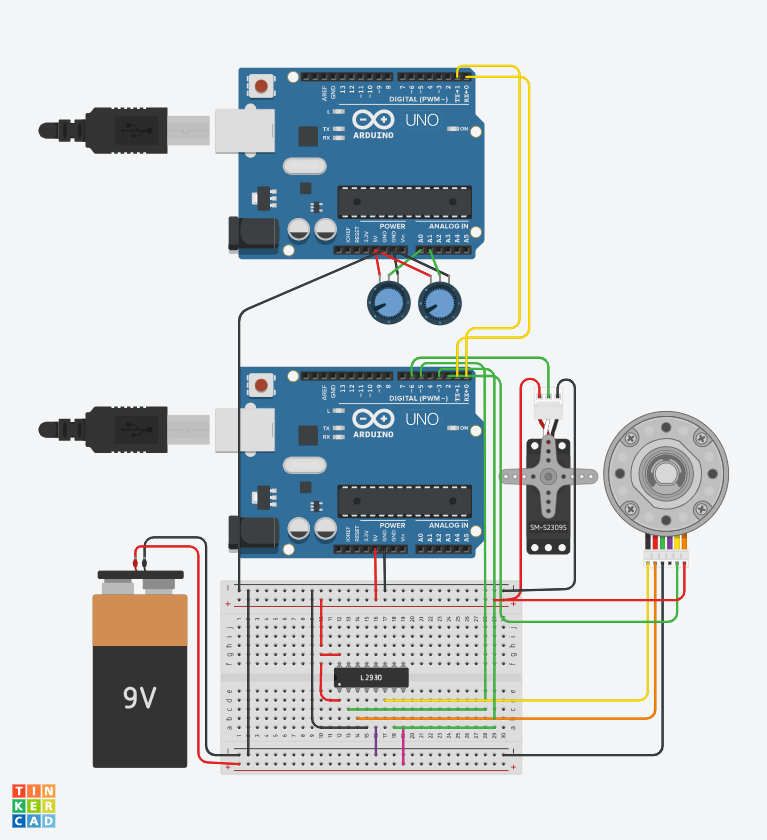
\includegraphics[width=16cm]{../../docs/car-hardware.png}}

You can see here two Arduinos, but on the car we only have one, why is that ? TinkerCad didn't have a Raspberry Pi, so we added another Arduino to simulate the serial connection between the Raspberry Pi and the Arduino. The Arduino on the top sends steering and throttle information (as the Raspberry Pi would do) to the other Arduino that processes this information received on the serial port and then controls both the servomotor and motor. They are both running on a 9V battery here but in real life on a 7.2V battery.
This virtual simplified car really helped us in the process of developing the core of our car !

When the Arduino part was finished, we could start the python part, that consisted in sending the right bytes to the serial port connected to the Arduino, it was hard to debug when there were issues on the one hand, but really satisfying when it did work ! We are now able to send steering and throttle to the Arduino making the car controllable using python !

% Ellerbach
\subsection{Camera}
The next step was to build a class to fetch images from our webcam, thankfully, the python module OpenCV has already some functions to do exactly that ! 
We only needed to add a wrapper around all of that to match our needs. We are now able to fetch images from our camera into a NumPy array that we can manipulate. On top of that, we did create a `dummy` version of this camera class in case we did not have access to a camera to run some tests, this class return a black image when we grab a new image form it. We use this class in some of our automated tests.

% Girold
\subsection{Load and save data}

% Gay
\subsection{Data set}
Previously, we created functions to load and save datas, those function handle json files and images. \\
Now we have to deal with data set but first, what is a data set ? \\ 
A data set is a folder which contains json files and images. Each file will have in its name the date followed by .png, the json should have the same name but it ends with .json instead of .png. In order to have the date, we have to use the time method time() which returns the time as a floating point number expressed in seconds since the epoch, in UTC.\\

Why dataset are so important ? \\ 
The goal of these part is to manipulate datat set. We take the information that the camera is giving to us and we can load, save and sort those datas in a cleaner way so that our training model and our Artificial inteligence model can use it.\\

We started by creating two files, the dataset.py file for the main functions and the test dataset.py in order to provide test functions to see if our code is working.\\

Firstly, for the dataset.py file, we had to import  two modules. \\
The first one is the glob module which finds all the pathnames matching a specified pattern according to the rules used by the Unix shell.\\
The second one is the OPS module. It provides functions for interacting with the operating system.\\

Secondly for the test file in addition to the module glob and os, we used the sys module. It provides access to some variables used or maintained by the interpreter and to functions that interact strongly with the interpreter.
We also used the shutil module which offers a number of high-level operations on files and collections of files. In particular, functions are provided which support file copying and removal. Furthermore, we used the numpy module to deal with matrices.\\


The dataset file is composed of ten functions :\\ 

The first is the load dataset function which load json and png file from a folder, the function takes the path of a directory which contains json and png and it returns a list of dictionnary containing the image and the json file.\\

The second function is the load multiple dataset, it is similar to the load dataset function but deals with multiple images and json files and it returns a list of list of dictionnary.  We also had a second argument named flat, if flat is equal to false,it means that we have to deal with a list of list, otherwise we have to deal with a simple list.\\

The third one is the load dataset generator function, it iterates image data, generators do not store all the values in memory, they generate the values on the fly.\\

The fourth one is the load multiple dataset generator. It is similar to the load dataset generator but it deals with several iamges and json files.\\

Then the load sorted dataset function sorts the loaded data and returns a list of ditionnary containing sorted data. Thanks to the function time.time() we have a chronogical view of our elements and we have to sort them. We had to use 2 subfunctions, the first is sort paths which sort all our elements thanks to the sorted function and the second subfunction is the get time stamp. The function split the name of an element in order to have only the part containing the date without the .json or .png  and then it convert it into a float.\\


The load multiple sorted dataset is similar to the load sorted dataset function but it deals with mutiple dataset and returns a list of list of dictionnary.\\

The two last function are the load sorted dataset generator and the load multiple sorted dataset generator.\\
It iterates sorted image data and do not store the values in the memory.\\



The test dataset file is composed of twenty-one functions.\\

We started to create the convert path function which is useful to convert path according to the current os because we encounter a major issue when we ran for the first time our test. Indeed, some errors appeared under Linux while under windows everythings works because the loading order is different under linux than under windows.\\ \\

Then we created the test sort paths is sorted function which test if the function  sortpaths returns sorted elements. \\

The third function is the test get time stamp. It test if the get time stamp function works, and if the value that it returns is a float. \\


Afterwards, we had to create a test directory to generate files containing image datas with an image, some datas like the steering and the throttle in order to test the other functions. \\

Firstly, we check if the number of files that we have created  is the same number present in the test directory. \\

Secondly, we check if the load dataset function was working using the previous files that we have created. We did the same test for the function load dataset generator. \\

Thirdly, we have to test if our functions are capabe to sort our dataset, by naming our files with different dates we can check if after the function load sorted datase we have a list of dictionnary in increasing order. \\

Afterwards, we created multiple directories and multiple files to test our function that take as parameters multiple directories. \\

We have types of function load multiple dataset, with have a flat version and a not flat version. \\
The difference is that for the flat version, datas are in the same folder and for the not flat version, datas are in different files. Our test are successful as we can collect our files independently of there folder. \\

We made the same test for the function test load multiple dataset generator not flat and for test load multiple dataset generator flat. \\

To finish, to get a cleaner work space, we delete all our folders created for those test. \\

% Ellerbach
\subsection{Data visualization}
In order to properly visualize our fetched data, we created some utils functions to do so.
The figure \ref{fig:a} shows a left turn and \ref{fig:b} a straight line.

\begin{figure}[h] 
    \centering
    \subfloat[Left Turn]{%
        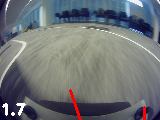
\includegraphics[width=0.49\textwidth]{../../docs/left-turn.png}%
        \label{fig:a}%
        }%
    \hfill%
    \subfloat[Forward]{%
        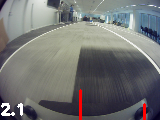
\includegraphics[width=0.49\textwidth]{../../docs/forward.png}%
        \label{fig:b}%
        }%
    \caption{An example of two visualized data}
\end{figure}

% Bobovitch
\subsection{Basic car loop}

% Girold
\subsection{Creation of the logo}

% Girold
\subsection{Realization of t-shirt}

% Bobovitch
\subsection{Website}


% sout : 7 / 03 & 25 / 04 & 06 / 06
\section {Planning}
\subsection {Races}

\begin{tabular}{|l|c|c|c|c|c|c|} 
\hline
Tasks & Race 1 & Race 2 & Race 3 & Race 4 & Race 5 & Race 6  \\ 
\hline
Code controlled motors and servo                & 75\%   & 100\%  &        &        &        &         \\ 
\hline
Drive the car with a controller                 & 25\%   & 100\%   &        &        &        &         \\ 
\hline
Data collection                                 &        & 50\%   & 100\%  &        &        &         \\ 
\hline
Telemetry website                               &        & 25\%   & 100\%  &        &        &         \\ 
\hline
Data processing and augmentation                &        &        & 50\%   & 75\%   & 100\%  &         \\ 
\hline
Basic Convolutional neural network              &        &        & 25\%   & 50\%   & 100\%  &         \\ 
\hline
\begin{tabular}[c]{@{}l@{}}Advanced \\models and optional objectives\end{tabular} &        &        &        &        &        & 50\%    \\
\hline
\end{tabular}

\subsection {Presentations}

\begin{tabular}{|l|c|c|c|} 
\hline
Tasks                                                                             & 1st presentation & 2nd Presentation & Final presentation  \\ 
\hline
Code controlled motors and servo                                                  & 100\%              &                &                    \\ 
\hline
Drive the car with a controller                                                   & 100\%              &                &                    \\ 
\hline
Data collection                                                                   & 75\%               & 100\%          &                    \\ 
\hline
Telemetry website                                                                 & 25\%               & 100\%          &                    \\ 
\hline
Presentation website                                                              & 100\%              & Update         & Update             \\ 
\hline
Data processing and augmentation                                                  &                    & 75\%           & 100\%              \\ 
\hline
Basic Convolutional neural network                                                &                    & 50\%           & 100\%              \\ 
\hline
\begin{tabular}[c]{@{}l@{}}Advanced \\models and optional objectives\end{tabular} &                    &                & 50\%               \\
\hline
\end{tabular}


\section {Task allocation}

\begin{tabular}{|l|c|c|c|c|} 
\hline
Tasks                        & Mickael B. & Maxime G. & Alexandre G. & Maxime E.  \\ 
\hline
Low level car control        &            &           &              & x          \\ 
\hline
Driving with a controller    &            & x         & x            & x          \\ 
\hline
Data storage and handling    & x          & x         & x            & x          \\ 
\hline
Telemetry website            & x          &           &              & x          \\ 
\hline
Presentation website         & x          &           &              &            \\ 
\hline
Convolutional neural network & x          & x         & x            & x          \\ 
\hline
Main control loop            & x          &           &              &            \\
\hline
\end{tabular}

\section {Conclusion}
To sum up, Autonomobile team improved the control of the car with controller, furthermore the data processing is working flawlessly allowing us to load and save images and metadata. Moreover, our presentation website is ready, it includes the presentation of the team, some links to download our project and even a road map. Nevertheless, the hardest part is yet to come, indeed we have to work on the AI part of the car and on the telemetry website to have it working by the next project defense. //
The telemetry website is important in order to visualize data to know what is happening inside the car at any moment. We will have to work and learn a lot on this topic which is fascinating. //

To make a long story short, we spent a lot of time on this project, which comport many sections that are important for the realization of this project, and we will do every thing to succeed. 


\end{document}
